%!TEX root = ../thesis.tex
%*******************************************************************************
%****************************** Third Chapter **********************************
%*******************************************************************************
\chapter{Optimising energy group structures for neutron activation calculations in fusion systems}
\label{chap:group_structure}

% **************************** Define Graphics Path **************************
\ifpdf
    \graphicspath{{Chapter3/Figs/Raster/}{Chapter3/Figs/PDF/}{Chapter3/Figs/}}
\else
    \graphicspath{{Chapter3/Figs/Vector/}{Chapter3/Figs/}}
\fi

% INTRODUCTION
%   Group structure optimisation literature review
%     Include a simple convergence study result
%   Self-shielding
%   Resonance behaviour: parameter correlations (matrix, resonance widths, f(Z,E))
%     Resonance Integrals, although structure, big resonances spread out over E-space
% METHOD
%   Nuclear data processing infrastructure
%     Pointwise ENDF
%     A Compact ENDF
%     Groupwise ENDF
%     Probability tables
%     Self-shielding factors
%   Energy group optimisation
%     Building a bin density distribution: rho(E) = SSF_{eff} + bpd_min
%     An iterative implementation
%   Radiation transport
%     Simple test case    # data on freia
%     JET model           
% RESULTS
%   Single optimisation: JET activation foils
%   Iterative optimisation: simple test case
% CONCLUSIONS / FURTHER WORK

\section{Outline}
\label{sec:outline}
% Update this

This study utilises self-shielding factors as a means to optimise energy group structures for fusion activation calculations. Informed by an analysis of important fusion resonances and a survey of relevant incident particle spectra, we develop and test two new group structures designed to more accurately represent the physics of nuclear reactions. They are compared to group structures commonly used in fusion research \& analysis. When used in a JET activation foil scenario, the optimised group structures outperform reference group structures, such as CCFE-709, while requiring fewer bins.

\section{Introduction}

Nuclear simulations for fusion devices are essential to determine material damage, activation-transmutation and to perform dose rate analyses. While continuous energy Monte Carlo modeling can be used to directly calculate reaction rates, due to the very large number (potentially tens of thousands) of possible reaction channels, it is impractical to compute all nuclear reactions of interest by this so-called point-wise approach. A separate inventory code, such as FISPACT-II \cite{fispact2015}, utilising a discretised incident particle spectrum is typically used to calculate all of these reaction rates, solve for the time-dependent nuclide inventory and provide various responses and source terms. This multi-group method is computationally efficient, but introduces self-shielding errors.

\subsection{Group structure optimisation}
% Greatly expand this...
The likelihood of interaction between an incident particle and a nucleus is a a non-linear function of energy in the resonant energy region. The cross-section, $\sigma(\mathrm{E})$ and the associated reaction rate, RR(E), may vary by several orders of magnitude within a few electron-volts. The number of bins that the energy domain is discretised over has a strong influence on the accuracy of the result. While increasing the number of bins increases the accuracy it also increases the time required to converge an input spectrum and the memory required to record this information\footnote{A concern for simulations with millions of voxels, common in activation-dose calculations.}. Figure~\ref{fig:gendf_convergence} shows a reaction rate converging to the true result as a function of the number of cross-section groups. These results are from a simple model where a 14 MeV point neutron source is located within a series of concentric, spherical shells made of steel, water and tungsten. The tallied reaction rate is radiative capture in \textsuperscript{186} in the outermost, tungsten shell. The neutrons are moderated by the water and the energy spectrum will receive sharp flux depressions from resonant nuclides within the steel material. This flux is then incident upon the tungsten where resonant peaks from the tungsten isotopes will further impinge on the spectrum. Without adequately resolving these depressions, an accurate estimation of the desired reaction rate cannot be made. In this example it can be seen that getting from a 10\% error to $\approx 1\%$ error requires a jump from 256 to more than 8192 bins. Any real problem will have many hundreds of nuclides present, with their nuclear data all discretised the same way, whether for a deterministic radiation transport calculation or an activation-transmutation calculation. Adopting such a fine discretisation for so many nuclides is not feasible given the memory requirements of such a scheme.

\begin{figure}[H]
  \centering
  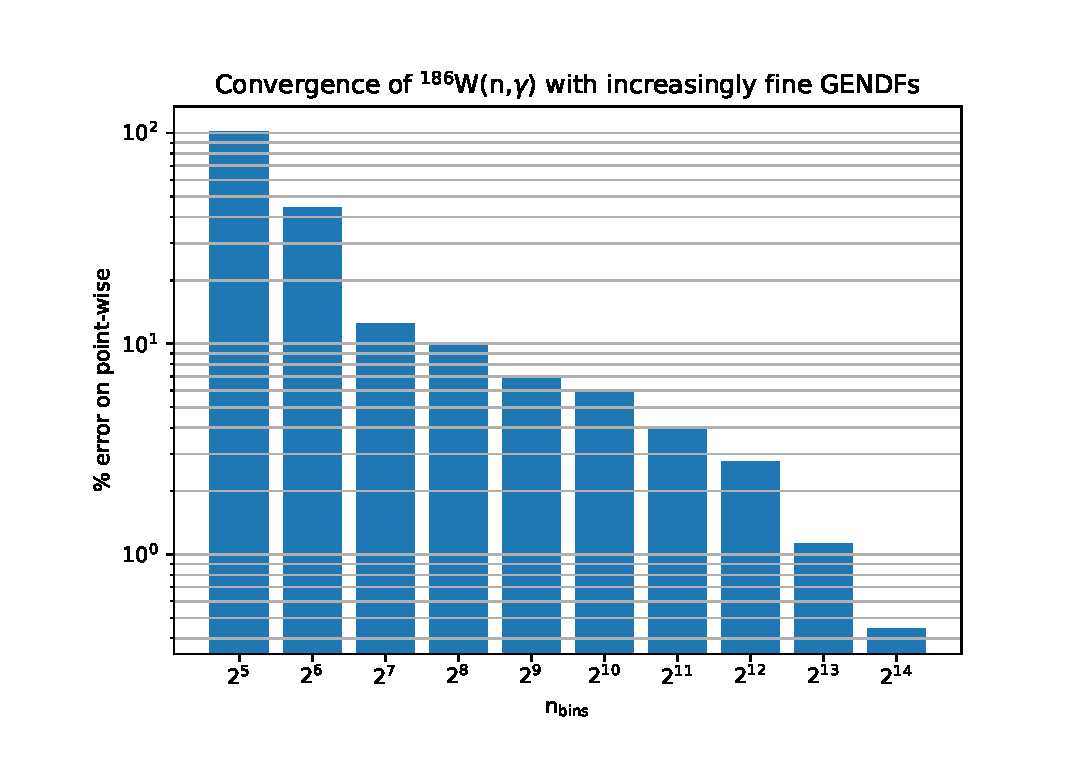
\includegraphics[width=0.9\linewidth]{gendf_convergence}
  \caption{This figure shows the results from a series of calculations with increasingly fine energy discretisations, or group structures. The bins for all groups are equally log-spaced. The calculation is to determine the (n,$\gamma$) reaction rate in a shell of \textsuperscript{186}W due to some incident neutron flux. The dependent variable is the \% change on a point-wise (true) value calculated with MCNP.}
  \label{fig:gendf_convergence}
\end{figure}

In addition to the number of bins, the bound locations have a strong relationship to the result accuracy. The integer bin count number and bound locations energy vector are together known as an energy group structure. In the example shown in figure~\ref{fig:gendf_convergence} the bin boundaries have been uniformally logarithmically distributed. This is a very simple starting point (and many group structures largely adhere to it) and can be improved upon, even if only to adopt one or two regions of different bin density.

% Expand this section, giving detail on each method
There have been several previous efforts to optimise neutron energy group structures. Certain applications lend themselves to highly targeted group structures. For example, fission reactor lattice physics calculations are typically interested in determining a few reaction rates to very high accuracy. The Studsvik team who develop the CASMO-5 lattice physics code employ a neutron group structure with very fine resolution around the principal $^{238}\mathrm{U}$ and $^{240}\mathrm{Pu}$ resonances \cite{Rhodes2006}. Covering these areas with a fine energy grid results in a more accurate estimate of key reaction rates and hence calculation of the neutrons absorbed and consequently lost from the system. Particle Swarm Optimisation (PSO) has been used multiple times to improve bin bound placement for multi-group libraries used for reactor physics applications \cite{Yi2013} \cite{Akbari2012} \cite{Akbari2013} \cite{Fleming2016}. \citet{Morgan2013} have explored hyperfine multi-group (MG) data as an alternative to the interpolation of point-wise (PW) data as typically employed by particle transport codes such as MCNP6.1 \cite{goorley2012}. Some attention has been directed towards the refinement of reaction rate calculation for specific elements and nuclides in fusion scenarios. For instance, work on the spatial heterogeneity of tungsten transmutation has been undertaken by \citet{Gilbert2016} who used the CCFE 709 bin group structure and careful application of self-shielding factors to accurately determine reaction rates.
% Comment on whether group structures are general or for specific applications. Can a general one ever be `optimised'? A: It is always a trade-off, generality vs. accuracy.

\subsection{Resonance behaviour}
% In terms of targeting group structure resolution, what can we learn from the distribution of resonance locations and widths?
It is clear that the placement of bin boundaries and the number of bins in an energy group structure has a significant effect on the potential accuracy of any calculation employing that group structure. The ideal location of these bin bounds is not some equal spacing, but more likely some complex result influenced by the kind of spectrum encountered and the nuclei present in the problem. This latter consideration can be explored by analysing the distributions of nuclear resonances for known nuclides within the \{A,E,j,$\Gamma$\} space, where A = atomic mass, $\mathrm{E}_{r}$ = interaction energy, j = nuclear spin and $\Gamma$ = resonance width. With knowledge of these distributions, especially in the mass and energy domains, perhaps energy bins might be targeted intelligently for a given problem.

To undertake this study, a set of scripts were written to parse resonance parameter information from nuclear data libraries. These can read ENDF-6 formatted entries, including several resonance formalisms for maximum nuclide coverage. The nuclear data library chosen to study was ENDF/B-VII.1 \cite{Chadwick2011}, the United States' reference nuclear data library. Figure~\ref{fig:res_energy_mass} is a scatter plot of 41,112 nuclear resonances from nuclides contained within this libary. 

\begin{figure}[H]
  \centering
  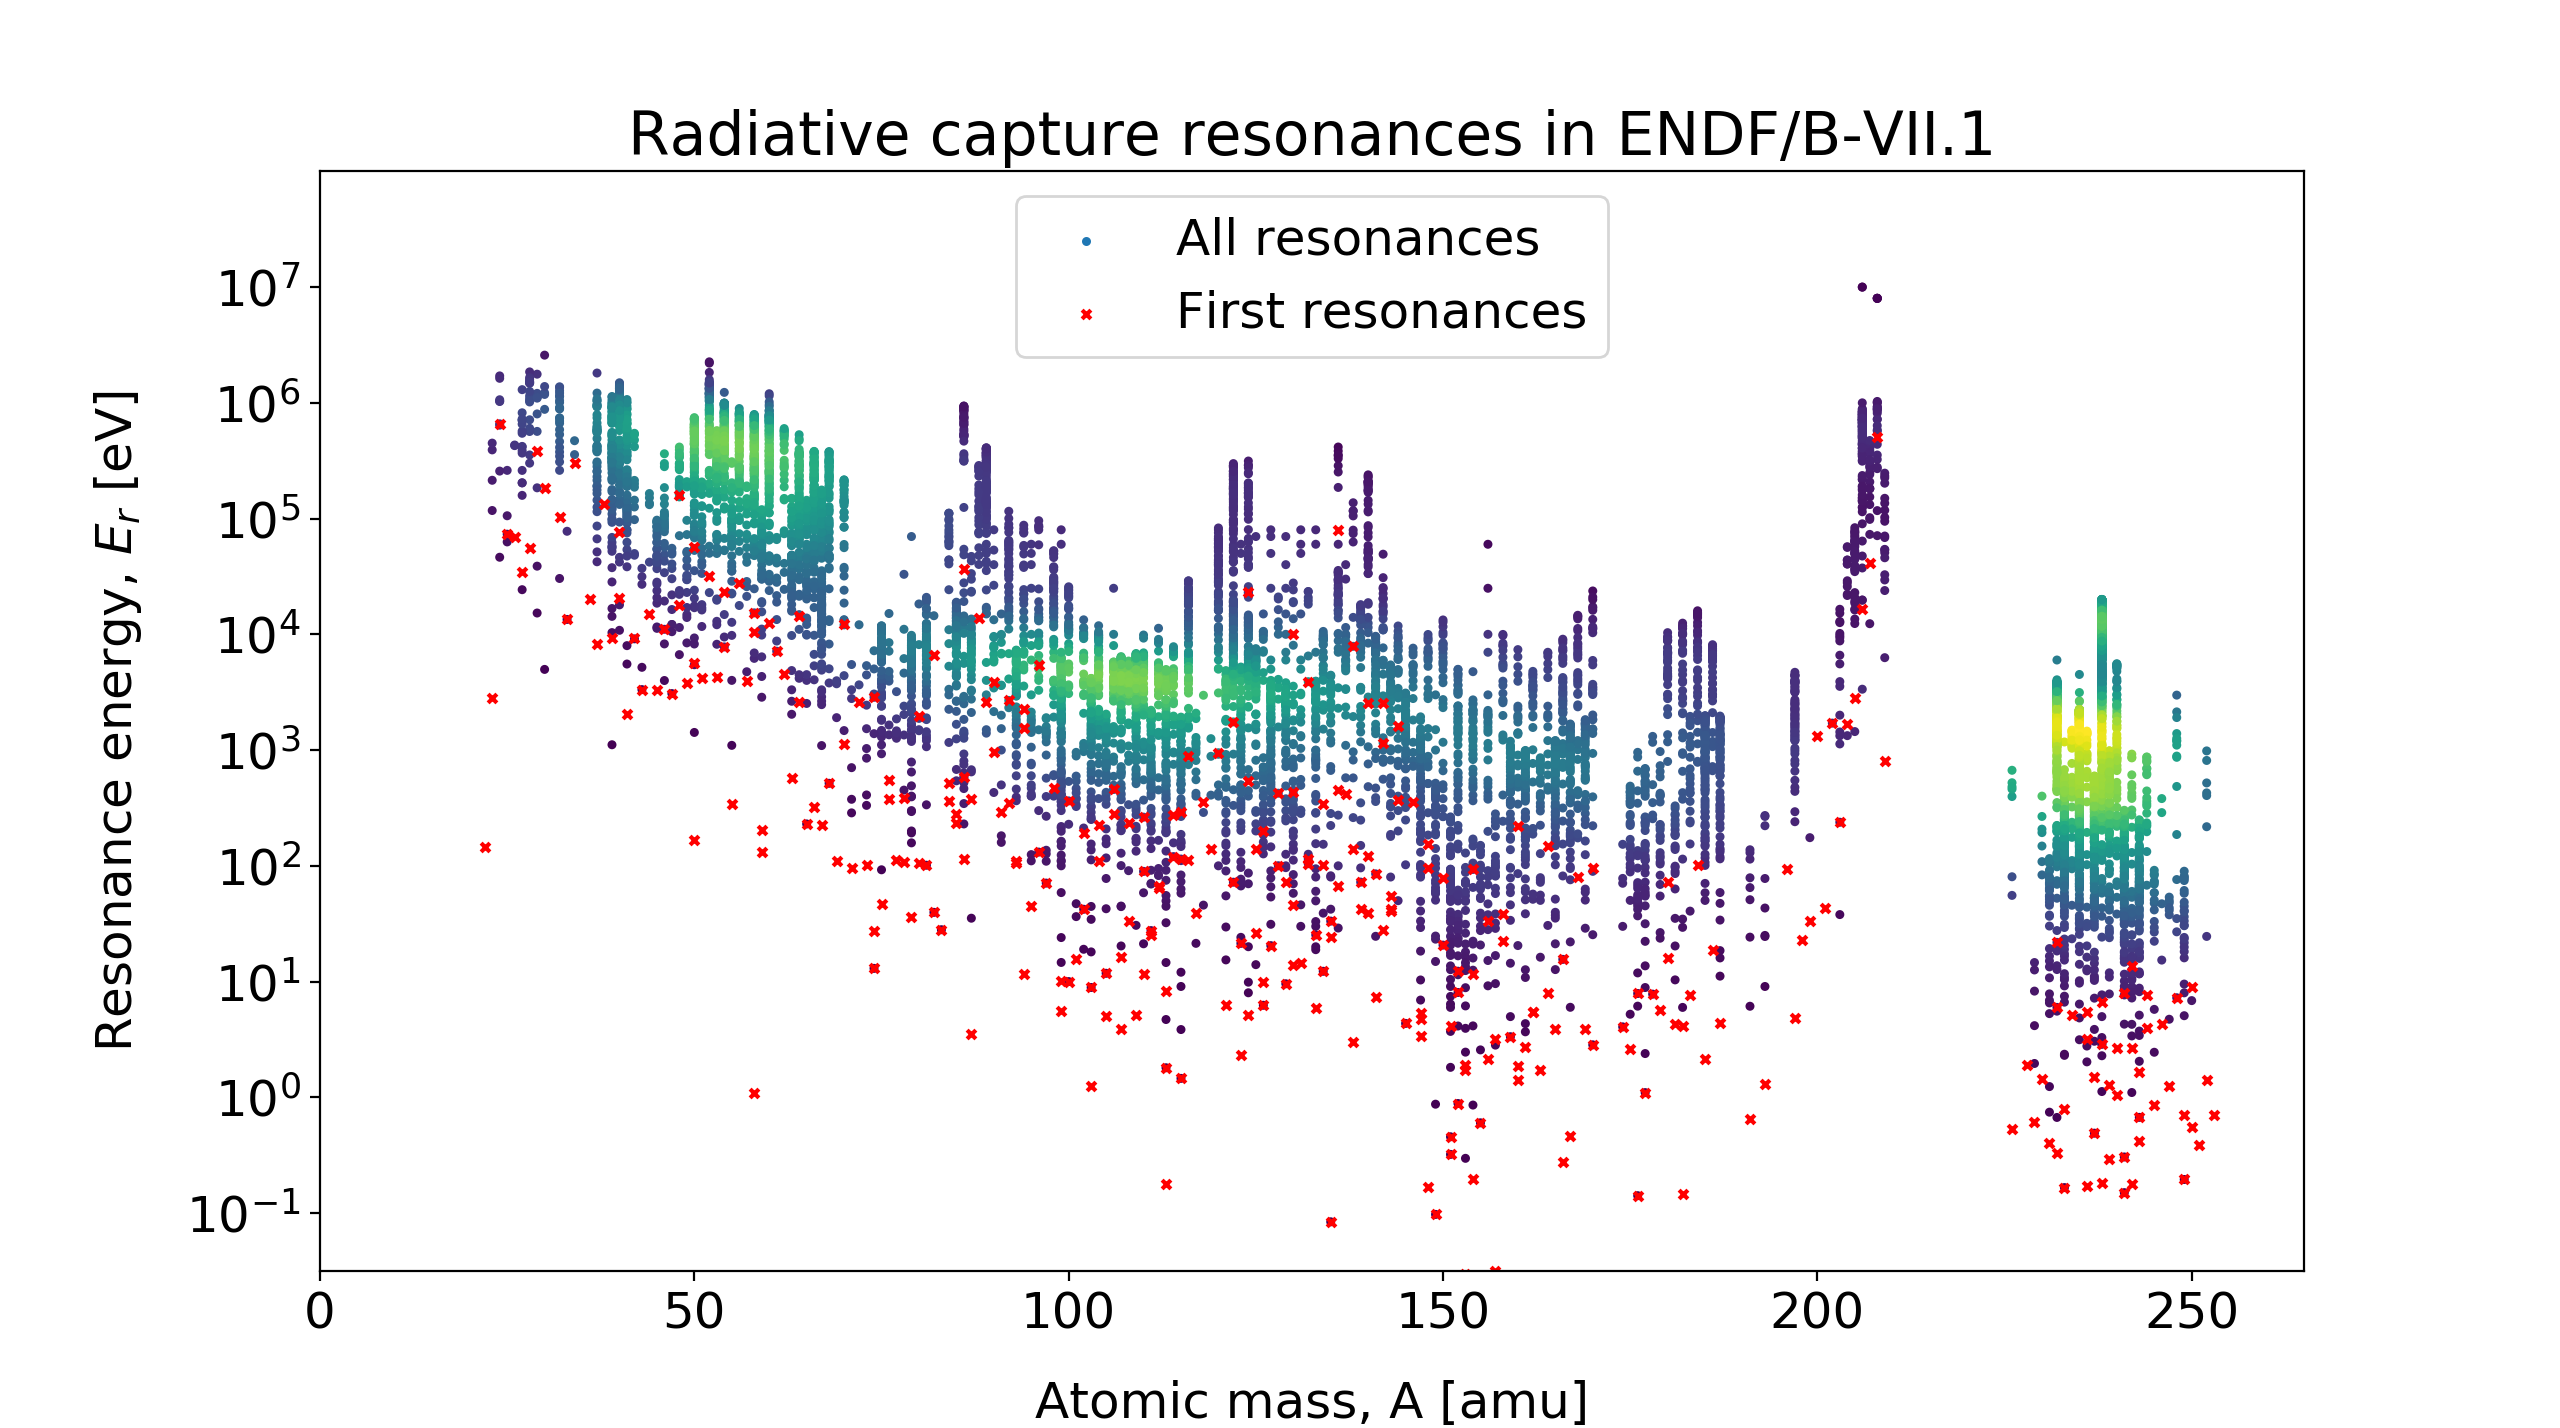
\includegraphics[width=\linewidth]{resonance_energy_atomic_mass}
  \caption{This scatter plot shows the energy of resonances as a function of atomic mass, for the majority of resonances recorded in the ENDF/B-VII.1 nuclear data library. The data are coloured by density, with blue as lowest density, green medium and yellow highest. The density has been calculated in \{log\textsubscript{10}(E), A\} space with a Kernel Density Estimator (KDE) approach. The first resonance for each nuclide is marked by a red cross for ease of identification.}
  \label{fig:res_energy_mass}
\end{figure}

Figure~\ref{fig:res_energy_mass} shows the general trend for lower energy resonances with increasing atomic mass. This trend is most pronounced up to $\mathrm{A} \approx 150$. After this point, the relationship flattens off for very large mass nuclides ($\mathrm{A} > 220$) and is completely invalidated for nuclides with $\mathrm{A} \approx 210$, the region of Pb \& Bi. Nuclides in this range are especially stable, close to the `magic numbers' of stable nuclei predicted by the nuclear shell model \cite{Stone1997}. Here, nucleons are especially tightly bound and a large energy input is required to reconfigure the nucleus. The highest density region is that of the actinides, where each nucleus has very many nuclear resonances, at comparatively low energies. Looking more generally, it can be seen that resonances are typically present for perhaps as much as 5 orders of magnitude of the energy spectrum for a given mass, a very large window. Taking all nuclides into account, resonances appear within the $10^{-1} < E_{r}\mathrm{[eV]} < 10^{7}$ range. If we assume that all resonances are equally important to consider when designing a group structure, then a fine grid might be required across this entire range, from practically thermal neutrons to unmoderated DT neutrons. 

\nomenclature[z]{KDE}{Kernel Density Estimator}
\nomenclature[z]{RI}{Resonance Integral}

% Need to introduce the concept of a resonance integral, refer back to BW description and describe our integration
We can quantify the `size' of a particular resonance by integrating a relevant descriptive function across some characteristic energy range, this so-called Resonance Integral (RI) is specified by equation~\ref{eq:res_integral}. 

\begin{equation}
  \label{eq:res_integral}
  RI = \int_{E_{r}-4\Gamma}^{E_{r}+4\Gamma} \frac{\pi\lambdabar^{2}(2J + 1)}{(2s_{n} + 1)(2s_{t} + 1)}  \frac{\Gamma_{i}\Gamma_{f}}{[(E-E_{r})^{2} + \Gamma^{2}_{t}/4]} dE
\end{equation}
% Very useful reference: http://www-pnp.physics.ox.ac.uk/~barra/teaching/resonances.pdf

Where $E$ is centre-of-mass energy of the system, $\Gamma_{i}$ is the partial resonance width to decay to the initial state, $\Gamma_{f}$ is the partial width to decay to the final state, $\Gamma_{t}$ is the total width, $\lambdabar$ the reduced particle wavelength, $E_{r}$ the rest mass energy of the resonance, $J$ the total angular momentum of the resonance, $s_{n}$ the neutron spin and $s_{t}$ the target spin \cite{Libby2005}. For formation of a compound nucleus by an incident neutron, leading to subsequent neutron emission, $\Gamma_{i}$ = $\Gamma_{f}$ = $\Gamma_{n}$, giving $\Gamma^{2}_{n}$ in the numerator. For radiative capture, it is instead $\Gamma_{n}\Gamma_{\gamma}$. 

RIs give an indication of the resonance's contribution to reaction rate. Computing the RI for all the resonances parsed in ENDF/B-VII.1 we can identify the largest and thus the most important to correctly represent in any energy discretisation scheme. These largest resonances are plotted as a function of energy in figure~\ref{fig:largest_res_energy_scatter}. Given these data are a subset of those presented in figure~\ref{fig:res_energy_mass}, many of the same trends as visible, such as the inverse relationship between energy and atomic mass. These largest resonance data do tend to be at the lower energy of the complete set and indeed further analysis shows that 20\% of the lowest energy neutron scattering resonances are also those with the largest RI for that nuclide. For radiative capture resonances, this figure is 41\%\footnote{The difference is because neutron scattering partial widths are correlated with interaction energy, whereas partial gamma widths are roughly constant (see figure~\ref{fig:res_correlation}).}. As such, it is not the case that the lowest energy resonances for each nuclide have always or even more often the largest RI. Any energy group structure optimisation routine should not simply target these resonances.

\begin{figure}[H]
  \centering
  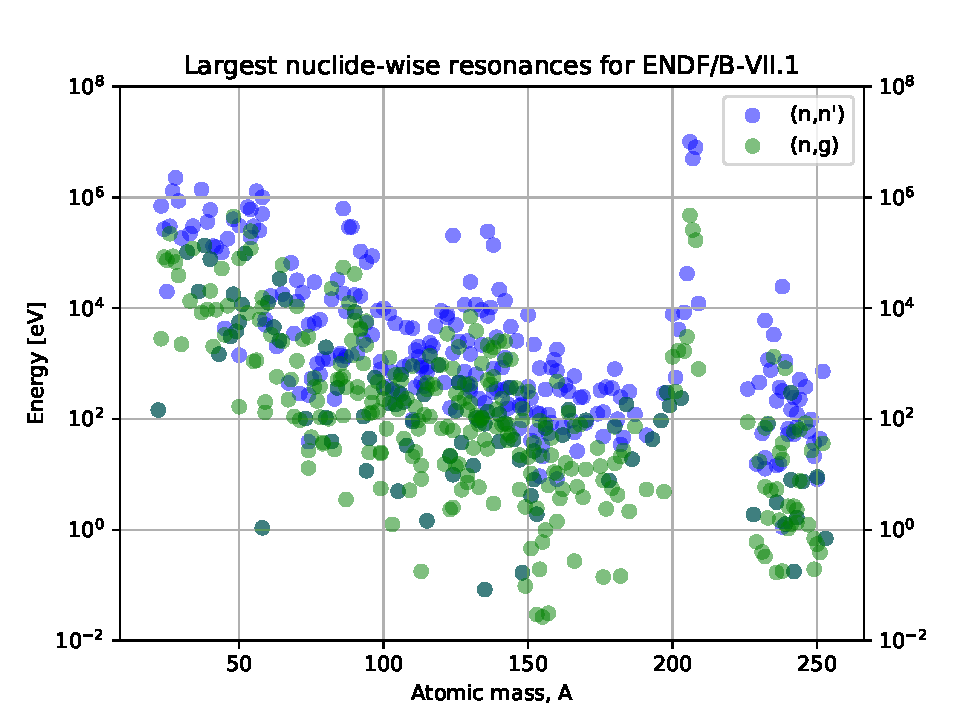
\includegraphics[width=\linewidth]{largest_res_energy_scatter}
  \caption{The energy of the largest resonances for ENDF/V-BII.1 as a function of atomic mass. The `largest' is determined by the RI as defined in equation~\ref{eq:res_integral}. Two datasets are shown, RI calculated using widths for neutron emission, $\Gamma_{n}$ in blue and for gamma emission, $\Gamma_{\gamma}$ in green.}
  \label{fig:largest_res_energy_scatter}
\end{figure}

It is instructive to inspect the correlations between various parameters recorded in the assembled resonance database. A correlation matrix of selected parameters is shown as figure~\ref{fig:res_correlation}. As previously shown in figure~\ref{fig:res_energy_mass} resonance energy and atomic mass are inversely correlated. $\Gamma_{n}$ is correlated with energy, while $\Gamma_{\gamma}$ is not. Given $\Gamma_{t} = \Gamma_{n} + \Gamma_{\gamma} + \Gamma_{f}$ but $\Gamma_{\gamma}$ is largely constant and $\Gamma_{f}$ is only important for a few resonances in particular nuclides, $\Gamma_{t}$ displays largely the same relations as $\Gamma_{n}$. 

\begin{figure}[H]
  \centering
  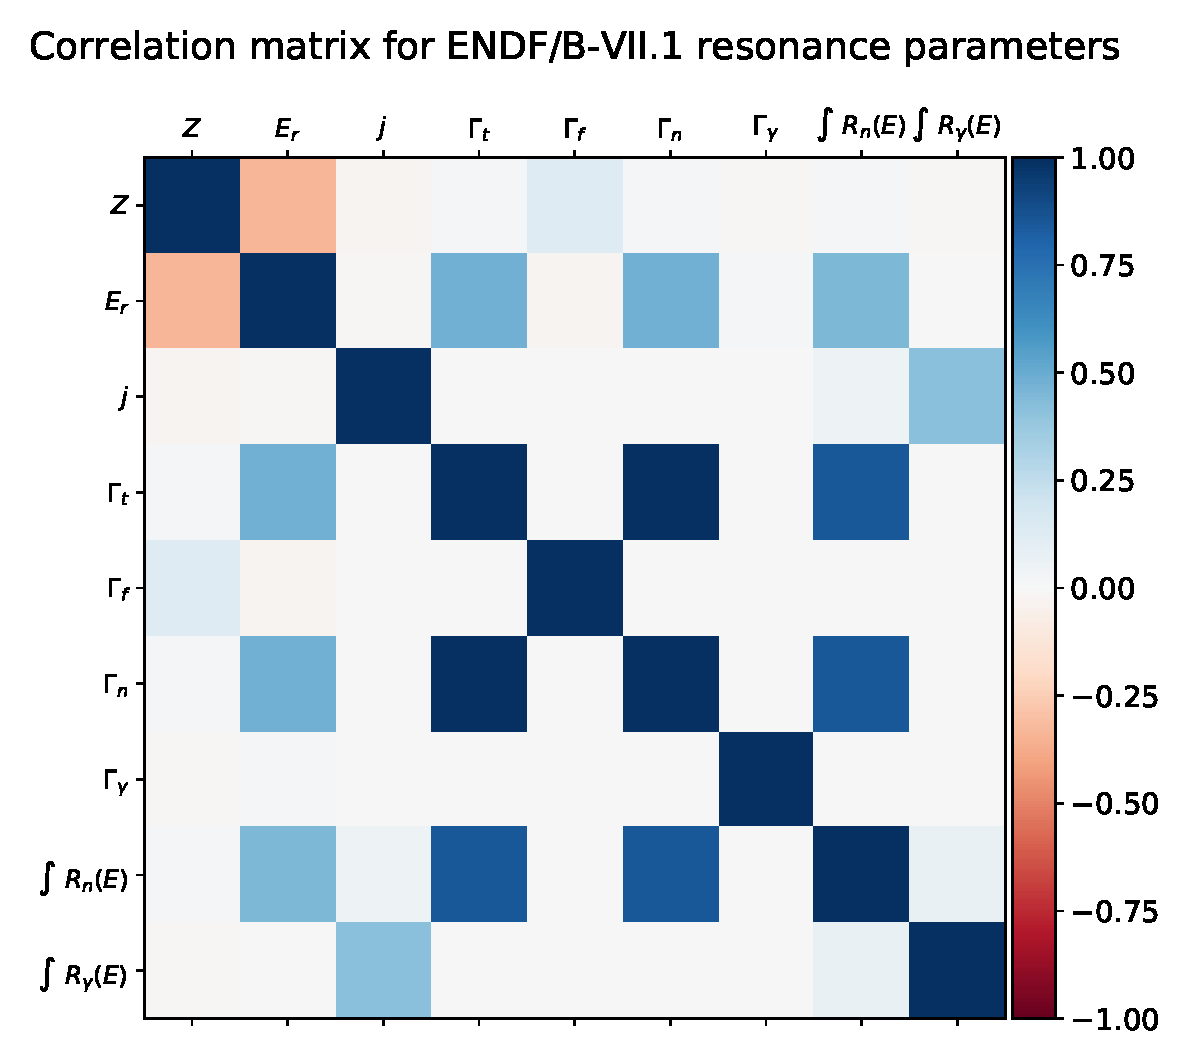
\includegraphics[width=\linewidth]{res_correlation}
  \caption{This correlation matrix is assembled from the resonance parameter data contained within the ENDF/B-VII.1 nuclear data library. It is constructed from the covariance matrix, showing how pairs of variables vary together, but normalised such that a meaningful comparison between relationships can be undertaken. The normalisation is given here \cite{numpy2018}. $A$ is atomic mass, $E_{r}$ resonance centre-of-mass energy, $l$ neutron orbital angular momentum, $J$ the total angular momentum, $\Gamma_{t}$ the total width, $\Gamma_{f}$ the fission partial width, $\Gamma_{n}$ the neutron emission partial width, $\Gamma_{\gamma}$ the $\gamma$-ray emission partial width, $\int R_{n}(E)$ the resonance integral for $\Gamma_{n}$ and $\int R_{\gamma}(E)$ the resonance integral for $\Gamma_{\gamma}$.}
  \label{fig:res_correlation}
\end{figure}

% So if we can determine which resonances are `biggest', how they are those ones inparticular distributed?
% Which features are there? 
% What causes them?
% Is any of this information useful to us?

% \begin{figure}[H]
%   \centering
%   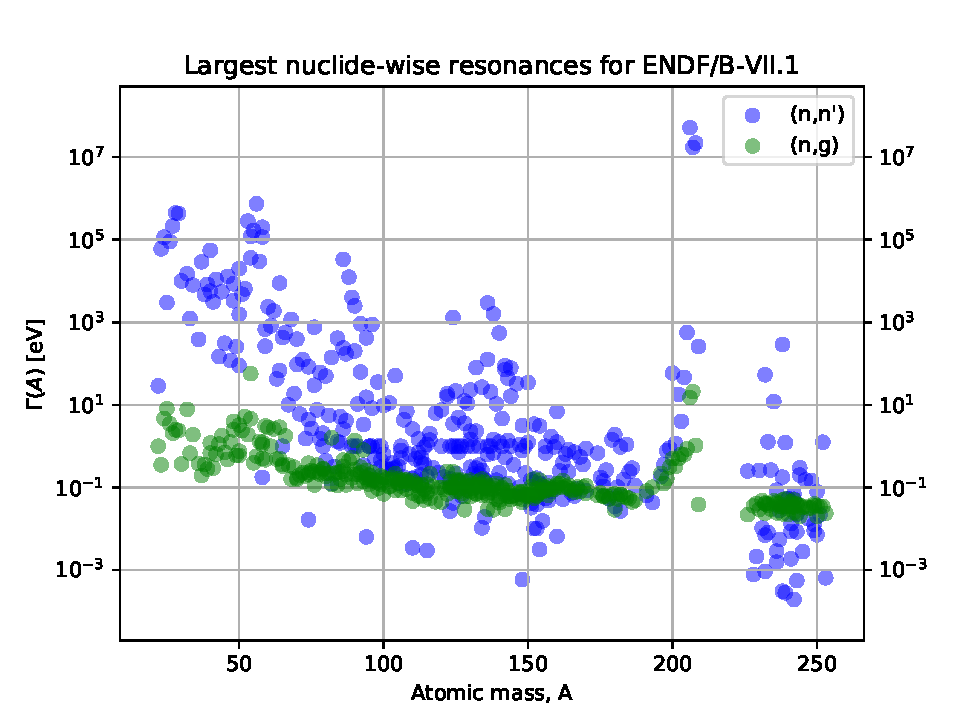
\includegraphics[width=\linewidth]{largest_res_width_scatter}
%   \caption{}
%   \label{fig:}
% \end{figure}

\subsection{Self-shielding}
\label{subsec:self-shielding}
The phenomenon of self-shielding is that whereby a particle flux is depleted in certain energy regions through absorption by the containing medium. This then `shields' the rest of the medium from those particle energies and decreases reaction rates. If this reduction in flux is not fed back then reaction rates will be overestimated. This effect is a particular problem where cross-sections and spectra are discretised into group-wise formats, as in deterministic radiation transport and activation-transmutation calculations. If energy groups are too large, flux depressions cannot be resolved.

Introducing \citeauthor{Bondarenko1964}'s self-shielding method exemplifies why a self-shielding treatment is necessary, how one can work and why it might be of interest for optimising group structures. 

Here we define an energy group, $E = [E_{0}, E_{1}, \dots, E_{G}]$ with $G$ groups. The lowest energy is $E_{0}$ and the highest $E_{G}$. The groups are in ascending energy order, so $E_{g+1} > E_{g}$, with the width of group $g$ given as $\Delta E = E_{g+1} - E_{g}$. To determine reaction rates, i.e. $RR(E) = N\sigma(E)\phi(E)$, where $N$ is the atomic density of the material, $\sigma(E)$ the cross-section and $\phi(E)$ the flux we need both the cross-section and the flux as a function of energy.

The flux for some group, $\phi_{g}$ is given by equation~\ref{eq:group_flux}.

\begin{equation}
  \label{eq:group_flux}
  \phi_{g} = \int_{E_{g}}^{E_{g+1}} \phi(E) dE
\end{equation}

We can define the group cross-section as equation~\ref{eq:group_cross_section}.

\begin{equation}
  \label{eq:group_cross_section}
  \sigma_{g} = \frac{\int_{E_{g}}^{E_{g+1}} \sigma(E) \phi(E) dE}{\int_{E_{g}}^{E_{g+1}} \phi(E) dE}
\end{equation}

$\sigma_{g}$ must be defined in such a way that it accurately reproduces the RR when multiplied by the flux. Unfortunately, equations~\ref{eq:group_flux} and \ref{eq:group_cross_section} require knowledge of $\phi(E)$ within a group, the quantity sought. If $\phi(E)$ were constant, then equation~\ref{eq:group_cross_section} would reduce to $\sigma_{g} = \int_{g}^{g+1} \sigma(E) dE$. While this is sometimes a reasonable assumption, if resonances are present in the group it is not. 

Looking for an expression to substitute for $\phi(E)$ we could first examine the total cross section of the system. Assuming a homogeneous mixture of M nuclides the total macroscopic cross section, $\Sigma_{t}$ is given by equation~\ref{eq:macroscopic_xs} where $N^{m}$ is the number density of nuclide $m$

\begin{equation}
  \label{eq:macroscopic_xs}
  \Sigma_{t}(E) = \sum_{m}^{M} N^{m} \sigma_{t}^{m}(E)
\end{equation}

The product of the energy varying flux, $\phi(E)$ and total macroscopic cross-section, $\Sigma_{t}(E)$ is the `collision density', $\phi(E) \Sigma_{t}(E) = S(E)$, or expressed equivalently as equation~\ref{eq:collision_density}.

\begin{equation}
  \label{eq:collision_density}
  \phi(E) = \frac{S(E)}{\Sigma_{t}(E)}
\end{equation}

If we let $S(E)$ be some smooth function, say a Maxwell-Boltzmann distribution or a 1/E particle slowing down spectrum, equation~\ref{eq:collision_density} shows us how the total cross-section impinges on the flux. A resonance within $\Sigma_{t}(E)$ causes $\phi(E)$ to drop, a flux depression. Substituting equation~\ref{eq:collision_density} into equation~\ref{eq:group_cross_section} gives the following:

\begin{equation}
  \label{eq:group_xs_s}
  \sigma_{g}^{m} = \frac{\int_{E_{g}}^{E_{g+1}} \sigma(E)^{m} \frac{S(E)}{\Sigma_{t}(E)} dE}{\int_{E_{g}}^{E_{g+1}} \frac{S(E)}{\Sigma_{t}(E)} dE}
\end{equation}

Equation~\ref{eq:group_xs_s} gives $\sigma_{g}^{m}$, the group cross-section for nuclide $m$, and can be used to generate all group cross-sections of interest for the problem if an appropriate $S(E)$ can be assumed. The macroscopic cross-sections on the right hand side of equation~\ref{eq:group_xs_s} are both total cross sections as any interaction will lower the flux. In the limiting case where the energy group width narrows to 0, $S(E)$ becomes constant, i.e. $\lim_{\Delta E \to 0} S(E) = k$ and $S(E)$ cancels from equation~\ref{eq:group_xs_s}. When energy group structures have a high bin density, they are reducing their reliance on this $S(E)$ function assumption.

The background cross-section is a concept introduced by \citeauthor{Bondarenko1964}. Cross-sections may belong to two mutually exclusive categories, they are either the cross-section of interest, or belong to a set `background' cross-sections which, if of sufficient magnitude act to depress the particle flux and shield the cross-section of interest. The macroscopic cross-section, $\Sigma_{t}(E)$ of equation~\ref{eq:macroscopic_xs} is then written as in equation~\ref{eq:background_xs}.

\begin{equation}
  \label{eq:background_xs}
  \Sigma_{t}(E) = N^{m} \sigma_{t}^{m}(E) + \sum_{n \neq m}^{M} N^{n} \sigma_{t}^{n}(E)
\end{equation}

We can factor out the number density for our nuclide of interest, $m$, to give equation~\ref{eq:background_factored}. 

\begin{equation}
  \label{eq:background_factored}
  \Sigma_{t}(E) = N^{m} (\sigma_{t}^{m}(E) + \sigma_{0}^{m}(E))
\end{equation}

Here $\sigma_{0}^{m}(E)$ is not a cross-section of nuclide $m$ in the normal sense, but all the cross-sections that contribute to its `background'. It is defined as equation~\ref{eq:background_xs_def}.

\begin{equation}
  \label{eq:background_xs_def}
  \sigma_{0}^{m}(E) = \frac{1}{N^{m}} \sum_{n \neq m}^{M} N^{n} \sigma_{t}^{n}(E)
\end{equation}

We can combine equations~\ref{eq:group_xs_s}, \ref{eq:background_factored} and \ref{eq:background_xs_def} to give equation~\ref{eq:group_xs_background}.

\begin{equation}
  \label{eq:group_xs_background}
  \sigma_{g}^{m} = \frac{\int_{E_{g}}^{E_{g+1}} \sigma^{m}(E) \frac{S(E)}{\sigma_{t}^{m}(E) + \sigma_{0}^{m}(E)} dE}{\int_{E_{g}}^{E_{g+1}} \frac{S(E)}{\sigma_{t}^{m}(E) + \sigma_{0}^{m}(E)} dE}
\end{equation}

The group cross-section for a given nuclide, $\sigma_{g}^{m}$, is a function of the background cross-section. 

Further detail on the above derivations are available in \cite{Dembia2013} \cite{Bell1970}. 

The calculation of reaction rates should incorporate the effects of self-shielding. As indicated above, a resonant material of particular interest to fusion plant designers is tungsten, with $^{186}\mathrm{W}(n,\gamma)$ shown in figure \ref{fig:w_cross_section}. This figure highlights the difficulties of determining reaction rates to a high accuracy. $^{186}$W has a large resonance at 18 eV and the energy-integrated reaction rate within this resonance typically dominates the total reaction rate. With the coarse group structure shown in the figure, an unshielded approach to computing the reaction rate yields values several times the `true' point-wise value. \citeauthor{Pampin2005} showed the importance of self-shielding for tungsten in fusion applications, finding that neglecting shielding effects can overestimate radiative capture in \textsuperscript{186}W by a factor of 6. \citeauthor{Gilbert2016}'s work built on this, sampling flux at multiple depths in first-wall tungsten to predict accurate rates of transmutation to rhenium and osmium. Even with this more sophisticated sampling, total unshielded reaction rates were sometimes twice their true value \cite{Gilbert2016}. Examples from the fission realm also abound, using a relatively coarse (but commonplace) 175 group structure \cite{Plechaty1978}, individual groups for \textsuperscript{232}Th cross-sections can be wrong by a factor of 50 \cite{Cacuci2010}. 

The self-shielding of resonant materials other than tungsten has yet to receive much attention in nuclear analyses of fusion power systems. A robust approach for accurately determining reaction rates for any material composition would be a welcome tool for future analyses. 

% Curse shielding, as in something to be minimised, but self-shielding theory and associated SSFs an opportunity for attacking the problem

%The rest of this paper details the first results of one approach, namely the intelligent discretisation of spectra and nuclear data to narrow important groups and make S(E) constant with E. Any remaining errors taken account of with self-shielding factors.

%\subsection{JET}

\section{Method}
\label{sec:method}

\subsection{Nuclear data processing}
% Describe infrastructure: design, robustness, testing, types of data
\subsubsection{Overview}
% Some sort of flowchart?

\subsubsection{Group structure}

\subsubsection{Point-wise ENDF}

\subsubsection{Group-wise ENDF}

\subsubsection{Probability tables}

\subsubsection{Self-shielding factors}

\subsubsection{A Compact ENDF}

\subsubsection{Data storage }

\subsection{Group structure optimisation}
\label{subsec:opt}

\subsubsection{Towards an ideal bin density function}
This study tests various group structures against a point-wise reference. We have generated two of the test group structures, attempting to optimise them to accurately calculate reaction rates for a set of nuclides.

To assemble a distribution for bin density we define several piecewise functions for identifying where, in the energy domain, self-shielding factor modifications are important and to indicate where resolution should be concentrated. 

Equation \ref{eq:s} describes the cumulative differences between reaction rates for an energy group as defined in section~\ref{subsec:self-shielding}. 

\begin{equation}
\label{eq:s}
S(E_{g}) = \sum_{i=0}^{g} \mathrm{RR}(E_{i}) - \mathrm{RR}(E_{i})\mathrm{SSF}(E_{i})
\end{equation}

The cumulative, effective self-shielding distribution,

\begin{equation}
\label{eq:c}
C(E_{g}) = 1 - \left( \left(1-\overline{\mathrm{SSF}}\right) \frac{S(E_{g})} {S(E_{N})}\right)
\end{equation}

begins at 1 for the first energy group, and to reduce to a minimum of the effective self-shielding factor $\overline{\mathrm{SSF}}$,

\begin{equation}
\label{eq:ssf_bar}
\overline{\mathrm{SSF}} = \frac{\sum_{g=0}^{N}\mathrm{RR}(E_{g})\mathrm{SSF}(E_{g})}
{\sum_{g=0}^{N}\mathrm{RR}(E_{g})}.
\end{equation}

This function, $C(E)$, gives a dimensionless measure of the importance of self-shielding modifications to interaction data. It allows comparison between nuclides of different cross-section values, as it is scaled between unity and the nuclide's $\overline{\mathrm{SSF}}$. Discontinuities in C(E) show regions with large effective self-shielding. An example of a cumulative SSF distribution is shown in figure \ref{fig:w_cross_section}. 

The differences between discrete elements of the cumulative distribution provide an effective self-shielding distribution,

\begin{equation}
\label{eq:d}
D(E_{g}) = C(E_{g}) - C(E_{g-1}),
\end{equation}

that identifies the relative contributions from each bin to the overall self-shielding effect. It is shown as the effective self-shielding distribution in figure \ref{fig:w_cross_section}.

As such, $D(E)$ indicates where the the group structure requires enhanced resolution in an improved group structure. However, outside the resonance ranges, for example for E $< 10^{-2}$ or E $> 10^{5}$ eV, this distribution is identically zero. To enforce a minimum bin density, a constant, $b$, is added to all bins of $D(E)$ in the algorithm employed. 

\begin{equation}
\label{eq:b}
b = \frac{D(E) \Delta E(E)}{\frac{n_{bins}}{bpd_{min}} - d}
\end{equation}

The minimum bins per decade, $\mathrm{bpd}_{min}$ must be specified. Where $d$ is the number of decades described by the group structure, $n_{bins}$ is the total number of bins required of the new group structure and $\Delta E(E)$ is an array of the input group bin widths.

\begin{equation}
\label{eq:offset}
\rho(E) = D(E) + b
\end{equation}

$\rho(E)$ is an array of proposed local bin densities, on the input group structure. This is then rebinned into equal areas as per equation \ref{eq:equal} to determine the new, optimised group structure.

\begin{equation}
\label{eq:equal}
\int_{g=i-1}^{g=i} \rho(E_{g})dE = \frac{1}{n_\mathrm{bins}}\int_{g=0}^{g=N}\rho(E_{g})dE \end{equation} 

The group structures tested in this study are listed in table \ref{tab:groups}. The two groups, 280 and 650, generated by our process were optimised for all stable nuclides of the following elements: Fe, W, Mo, Nd, Sn, Zr, Cu, Co and Ta. This means we performed the nuclide-wise integral of $\rho(E)$ for all naturally occurring isotopes of these elements. 

\begin{table}[H]
  \centering
  \begin{tabular}{lllll}
    \toprule
    n$_\mathrm{bins}$ & E$_\mathrm{min}$ (eV) & E$_\mathrm{max}$ (eV) & bpd$_\mathrm{res}$ & Description \\ 
    \midrule
    709 & 1E-5 & 1E9 & 50 & CCFE \\
    650 & 1E-5 & 1E8 & 37--101 & Optimised fine \\
    315 & 1E-5 & 1.94E7 & 24--50 & TRIPOLI  \\
    280 & 1E-5 & 1E8 & 11--73 & Optimised coarse \\ 
    175 & 1E-5 & 1.96E7 & 5--22 & VITAMIN-J \\
    \bottomrule
  \end{tabular}
  \caption{Comparison of group structures tested, noting their bin counts, n$_\mathrm{bins}$, the energy range over which they are defined and the bins per decade, bpd$_\mathrm{res}$ they employ in the resonant region.}
  \label{tab:groups}
\end{table}

\subsubsection{Iterative and other methods}
% Iterative application but also coarsening approaches – all still using some form of rho(E)

\subsection{Computation}

The calculation of effective cross-sections were carried out using three different techniques:

\begin{enumerate}
  \item Multi-group FISPACT-II unshielded collapse
  \item Multi-group FISPACT-II shielded collapse
  \item Point-wise MCNP6 Monte Carlo Estimator (MCE)
\end{enumerate}

Methods 1 \& 2 discretise the incident spectrum, over a  $\phi(E)$ and $\sigma(E)$, taking the inner product of two vectors of constants,
$$\vec{\phi} \cdot \vec{\sigma} = \sum_i \phi(E_i , E_{i+1}) \sigma(E_i , E_{i+1}),$$
as the spectrum-averaged, effective cross section. However, for each group interval, $(E_{i}, E_{i+1}]$ the true functions $\phi(E),\ \sigma(E)$ are not contant. Regions with resonances in the cross section cause local decreases in the neutron flux, resulting in significant `self-shielding' errors with the multi-group method. To address this, self-shielding factors, $\mathrm{SSF}(E_i)$, may be used to account for these resonance effects. 

An incident spectrum, material inventory and nuclear data are input to FISPACT-II. The spectrum and interaction nuclear data are then collapsed to generate one-group effective cross-sections. With the addition of probability table data generated with CALENDF-2010 \cite{sublet2011}, $\mathrm{SSF}(E_i)$ are calculated for both the resolved and unresolved resonance regions.

Method 3 employs nuclear cross-section data with tens of thousands of points per reaction channel, interpolating between them to approximate a continuous energy treatment. The effective radiative capture cross-section can be determined from the point-wise calculated $(n,\gamma)$ reaction rate as equation \ref{eq:pw}. 

\begin{equation}
\label{eq:pw}
\sigma_\mathrm{eff} = \frac{\int RR_{n,\gamma}(E) dE}{\int \phi(E) dE}
\end{equation}


The effective cross-sections calculated for this study were a series of radiative capture reactions in metals. These reactions often have a large fraction of their total reaction rate within the neutron slowing down region between thermal and fast energies. Hence, an accurate resonance treatment is required for accurate results. 

\subsubsection{Simple test case}
% Concentric spheres used in iterative method, give description of geometry, data and radiation transport

\subsubsection{JET activation foils}

The radiation transport geometry utilised in this study is the JET tokamak located near Abingdon, Oxfordshire. Octant 8 of the tokamak has previously housed the Long Term Irradiation Station (LTIS) for exposing activation foils to the JET neutron field. A variety of $(n,\gamma)$ effective cross-sections have been calculated in various materials and for a selection of energy group structures. Some of these group structures are optimised for the materials present in the simulation, while others are standard group structures in common usage today. 

\begin{table}[h]
  \centering
  \begin{tabular}{lll}
    \toprule
    Reaction                                       & E$_\mathrm{first\ res.}$ (eV) & E$_\mathrm{URR}$ (eV) \\ 
    \midrule
    %%$^{58}\mathrm{Fe}(n,\gamma)^{59}\mathrm{Fe}$   & 2.29E2                        & 3.50E5                 \\
    %%$^{59}\mathrm{Co}(n,\gamma)^{60}\mathrm{Co}$   & 1.31E2                        & 1.19E5                \\
    $^{95}\mathrm{Mo}(n,\gamma)^{96}\mathrm{Mo}$   & 4.47E1                        & 5.87E4                \\
    $^{181}\mathrm{Ta}(n,\gamma)^{182}\mathrm{Ta}$ & 4.27E0                        & 4.00E3                \\
    $^{182}\mathrm{W}(n,\gamma)^{183}\mathrm{W}$   & 4.16E0                        & 9.91E4                \\
    $^{186}\mathrm{W}(n,\gamma)^{187}\mathrm{W}$   & 1.88E1                        & 1.21E5                \\ 
    \bottomrule
  \end{tabular}
  \caption{Shown above are the reactions simulated in this study. E$_\mathrm{first\ res.}$ indicates the energy of the first resonant peak in the interaction cross-section. E$_\mathrm{URR}$ defines the end of the resolved resonance range (RRR) and the start of the unresolved resonance range (URR) where experimental energy resolution is insufficient to resolve individual resonances.}
  \label{tab:reactions}
\end{table}

The reaction channels chosen for study are listed in table \ref{tab:reactions}. The nuclides listed are found in the designs of fusion power systems; iron is the principal constituent of all steels, cobalt a steel impurity which dominates shut down dose rates at intermediate time scales, molybdenum an important steel alloying element, tantalum is being investigated for use in high-heat flux componentry and tungsten is a current first choice for a plasma facing high-heat flux material.

In order to compare the performance of the different group structures, incident particle spectra were obtained. As previously mentioned, the LTIS foil holder is located within Octant 8 of the JET facility. The LTIS MCNP model \cite{lengar2017} was integrated into a reference JET model. The LTIS was populated with foils of the materials noted in table \ref{tab:reactions}. The simulation was set to tally the reaction rates of interest in each of the foils in each specified group structure. Point-wise tallies were also included.

\section{Results \& Discussion}
\label{sec:results}
% Introduce general approach again, tall plot of SSF effect functions is to follow

%%To generate self-shielding factors using FISPACT we require a spectrum. The spectrum shape guess was $\phi(E) = E^{0.192}$, or slightly harder than `flat' (see figure \ref{fig:spectrum} for an indication of the spectrum). 
% Include this test spectrum plot, and the lin-log profile used to bias the SSFs

\subsection{Singly optimised}

\begin{figure}[H]
  \centering
  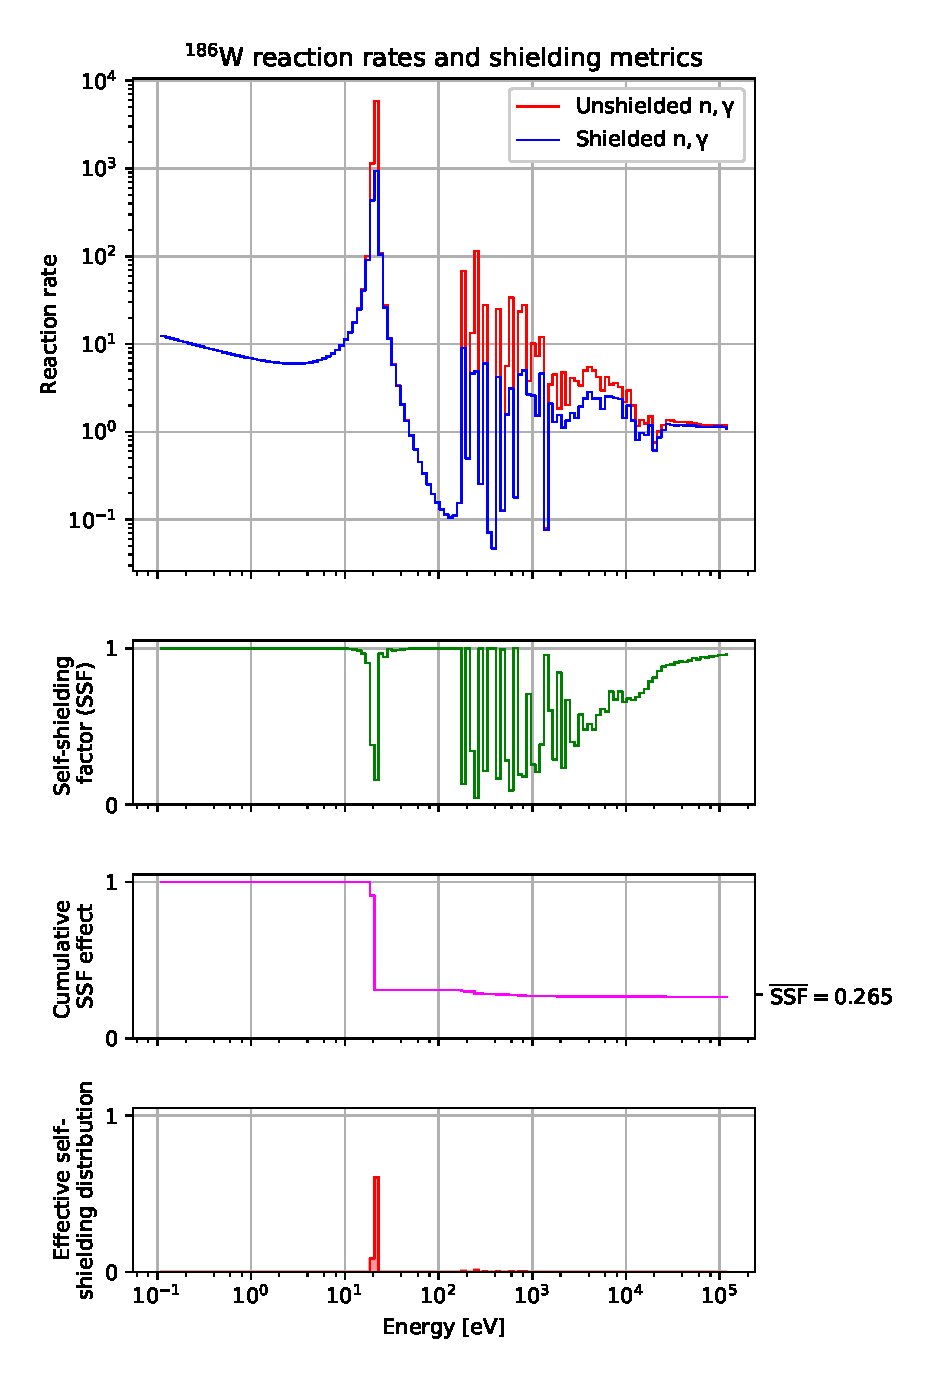
\includegraphics[width=0.8\linewidth]{W186_gamma}
  \caption{Shown in the upper plot is a $^{186}$W radiative capture reaction rate, both unshielded and shielded. The incident particle spectrum in this case is a power function of energy, i.e. $\phi(E) = E^{x}$ where $x$ is some constant. The second plot shows the calculated self-shielding factors as a function of energy for this reaction, given an elemental material composition. The third and fourth plots are derived quantities used for group structure optimisation.}
  \label{fig:w_cross_section}
\end{figure}

A set of sample LTIS spectra are as shown in figure \ref{fig:spectrum}. These particular spectra are from within the tungsten foil. Resonances both within the tungsten and the surrounding materials have resulted in flux depressions. An expanded view of the $^{186}$W 18 eV resonance is shown as figure \ref{fig:spectrum_detail}. The degree to which the resonances are resolved by the different group structures is a function of the bin resolution around the resonance. The 709 group, with a standard 50 bins per decade reaches down into the 18 eV resonance, recording a fluence of 3.5E-9 whilst the optimised group structures, 280 and 650 record 2.32E-9 and 1.26E-9. The standard group structures 175 and 315 which are much coarser in this region record a minimum fluence more than an order of magnitude greater than the 650 group structure.

\begin{figure}[H]
  \centering
  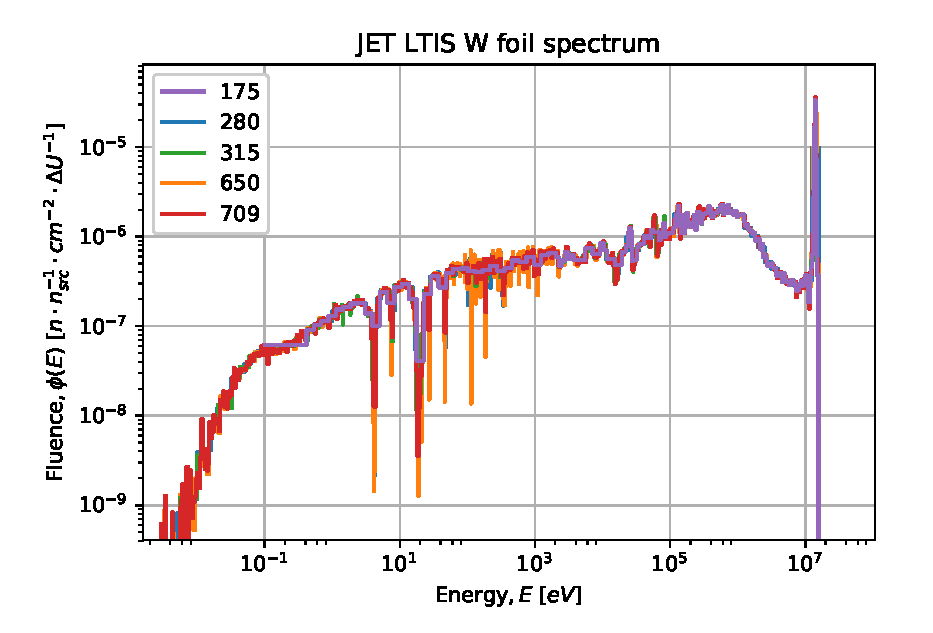
\includegraphics[width=\linewidth]{W186_spectra_diff_groups.eps}
  \caption{Typical DT neutron spectrum within the LTIS activation foil holder. The fluence of each bin has been divided by the lethargy width for that bin, $\Delta U$. The spectrum is hard, with little thermalisation as a consequence the foil's proximity to the plasma. The same neutrons have been binned according to various group structures, from 175 to 709 groups.}
  \label{fig:spectrum}
\end{figure}

\begin{figure}[H]
  \centering
  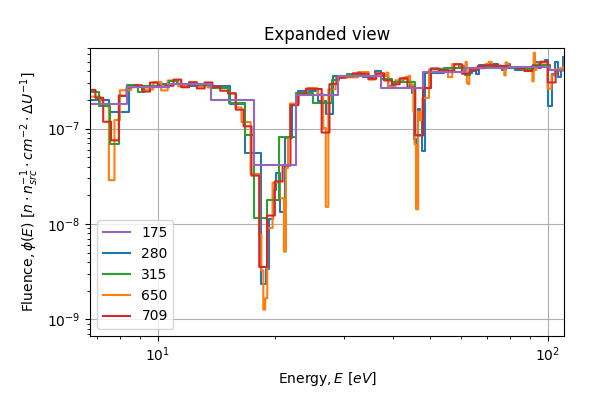
\includegraphics[width=\linewidth]{w_spectrum_detail}
  \caption{Magnified section of spectrum showing how progressively finer group structures resolve flux depressions in a neutron spectrum.}
  \label{fig:spectrum_detail}
\end{figure}

Figure \ref{fig:tungsten-182} shows a comparison of collapsed cross-sections for $^{182}$W. The abscissa lists each group structure tested. A pair of data points exist for each group structure, one with the use of self-shielding factors (shielded) and one without (unshielded). The abscissa order is a sorted such that the unshielded values decrease from left to right. The left ordinate indicates the absolute cross-section value in barns, while the right ordinate gives the cross-section as a percentage change over the point-wise (reference) value, i.e. +100\% means the multi-group calculation has over-estimated the cross-section and therefore reaction rate by a factor of 2.

As would be expected, in a simple, unshielded case having more groups and therefore a larger number of groups per energy decade tends to give multi-group results closer to the reference point-wise result. Flux depressions are better resolved with narrower groups and therefore the reaction rate resulting from resonances is not overestimated to the same degree. However, with the exception of $^{181}$Ta, the 650 optimised group, and even the 280 optimised group perform better than the 709 group in the unshielded regime. Their narrow groups are targeted where most useful, around the resonances which were poorly described by a equal logarithmically spaced group structure.

\begin{figure}[H]
  \centering
  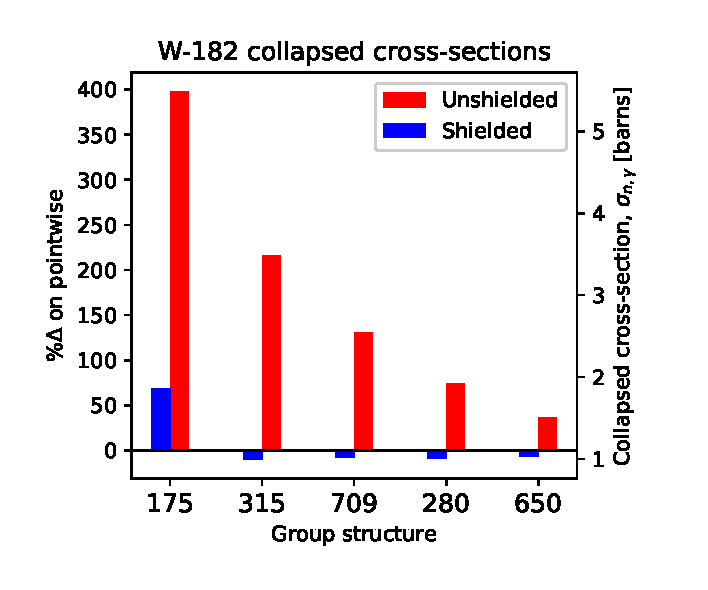
\includegraphics[width=\linewidth]{W-182.eps}
  \caption{Comparison of different calculation methods for radiative capture in $^{182}$W under JET neutron irradiation.}
  \label{fig:tungsten-182}
\end{figure}

With regards to individual groups, the 175 group used unshielded performs very poorly, overestimating the reaction rate by at least a factor of 3 in all cases. The 650 optimised group is always within 50\% of the point-wise result and is the best performing group.

\begin{figure}[H]
  \centering
  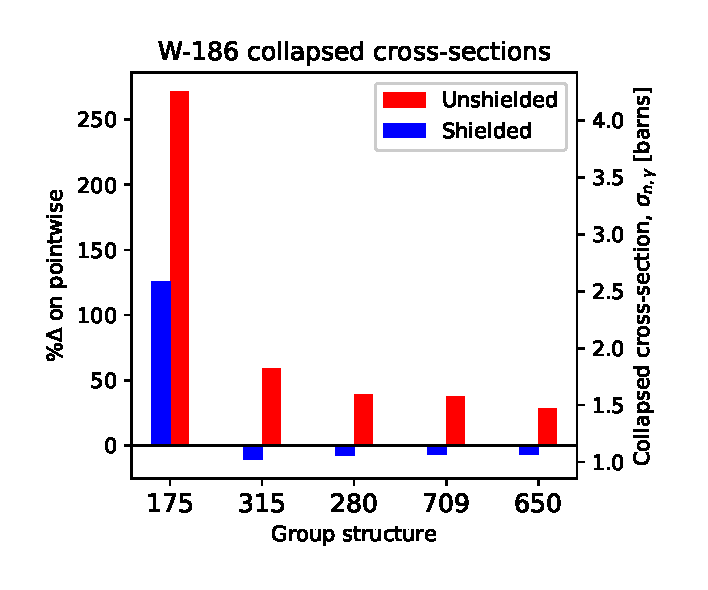
\includegraphics[width=\linewidth]{W-186.eps}
  \caption{Comparison of different calculation methods for radiative capture in $^{186}$W under JET neutron irradiation.}
  \label{fig:tungsten-186}
\end{figure}

As might be expected the shielded results show far less variation between groups. 280, 315, 650 \& 709 demonstrate largely similar behaviour when used in conjunction with self-shielding factors. 175 does again over-estimate, between 0\% and 120\% depending on the nuclide.

\begin{figure}[H]
  \centering
  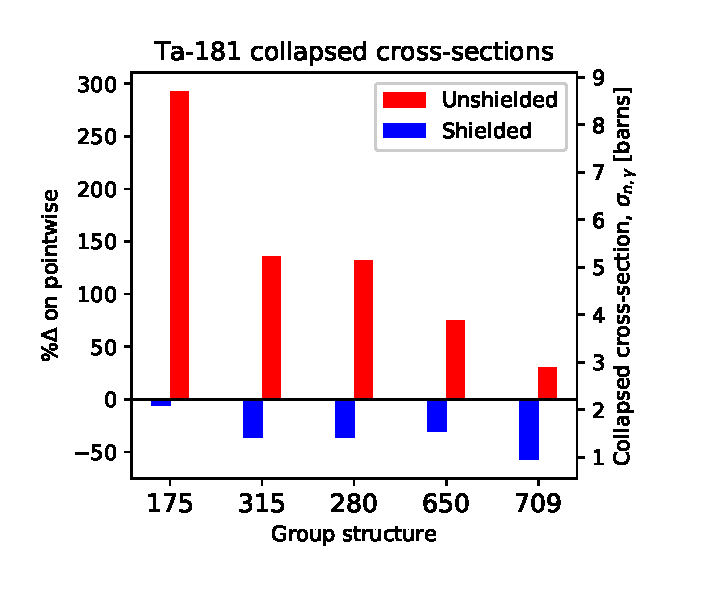
\includegraphics[width=\linewidth]{Ta-181.eps}
  \caption{Comparison of different calculation methods for radiative capture in $^{181}$Ta under JET neutron irradiation.}
  \label{fig:tantalum-181}
\end{figure}

The $^{181}$Ta (figure \ref{fig:tantalum-181}) and $^{95}$Mo (figure \ref{fig:molybdenum-95}) results indicate over-shielding, that is self-shielding factors over compensating for a poor description of the spectrum. This is particularly pronounced for the 315 group in $^{95}$Mo, where the shielded result is 40\% less than the point-wise result. This is due to the application of one set of self-shielding factors over the entirety of the foil depth. Although only 500 microns, the compound geometric effects are essential and are the subject of further work.

\begin{figure}[H]
  \centering
  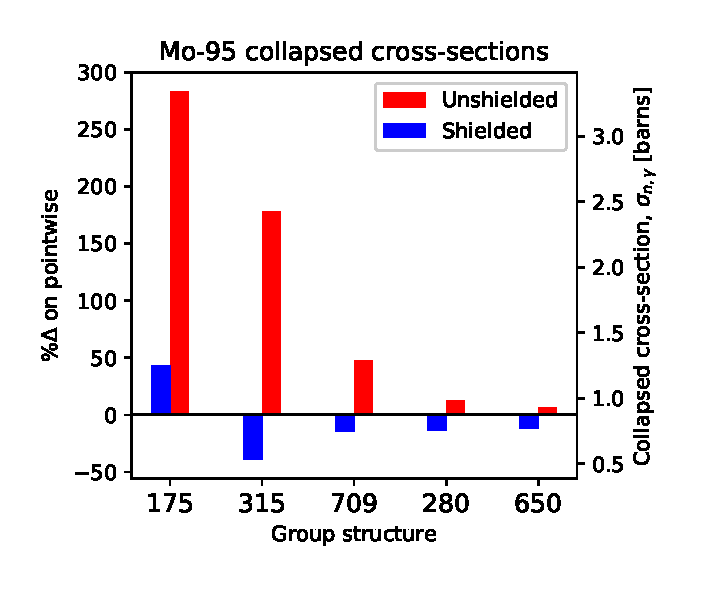
\includegraphics[width=\linewidth]{Mo-95.eps}
  \caption{Comparison of different calculation methods for radiative capture in $^{95}$Mo under JET neutron irradiation.}
  \label{fig:molybdenum-95}
\end{figure}

\subsection{Advanced methods}
% Results from iteratively applying algorithm, coarsening vs. straight rho(E), etc.


\section{Conclusions}

This study has investigated how an incident spectrum and nuclear data library are discretised in energy (i.e. the group structure) effects the accuracy of reaction rate calculations. The selection of group structures trialled included three in current use and two which were optimised by our own, novel method.

The accuracy of multi-group reaction rate calculations is severely hampered by using the legacy VITAMIN-J 175 group structure. In the context of this activation foil problem, coarse group structures can give reasonable results if used in conjunction with modifying self-shielding factors. If used, self-shielding factors must be applied carefully, with potential geometric shielding effects considered. If used inappropriately, over-shielding may result, which may not be conservative depending on the context.

An optimisation algorithm has been demonstrated. The algorithm can generate and optimised set of bin bounds, given a `guess' spectrum and a target nuclide set. An unshielded multi-group calculation using an optimised group structure with 280 bins has more closely approximated the point-wise result than the 709 unshielded multi-group calculation in the majority of cases examined.

Further work will improve on the optimisation algorithm and explore the performance of optimised group structures in a wider array of circumstances. Iterative application of the algorithm will be investigated as well as geometric self-shielding effects. 

